Sensitivity analysis identifies how the variation of model input
parameters affect select performance 
metrics of the fuel cycle. Additionally, it reveals the combined effect 
of varying multiple parameters on 
an output metric. This information is then used to design 
an optimized transition scenario by identifying which input parameters 
will affect the results the most, and how these parameters should be 
changed to obtain desired results (e.g., minimizing \gls{HALEU} requirements
of a transition). 

\section{Methodology}
The analysis was performed on Scenario 7 and Scenario 
14 to provide insight into how the input parameters affect the output 
metrics for both a once-through and recycle fuel cycle. 

\Cyclus was coupled to Dakota \cite{adams_dakota_2019},
and Dakota is the driver for the analysis. This coupling mirrors  
the scripts in the \texttt{dcwrapper} GitHub repository \cite{chee_arfcdcwrapper_2019}.
Three different types 
of sensitivity analysis were performed: \acrfull{OAT}, synergistic, 
and global. \gls{OAT} analysis varies a single input parameter to 
investigate the effect of each parameter individually. In the context of 
this work, synergistic 
analysis varies two input parameters at once to investigate how the 
interaction of the two parameters affects the results. Finally, the global 
analysis varies more than two input parameters to provide a holistic 
view of how multiple parameters interact and affect the output metrics. 

The input parameters varied include the transition 
start time, the build share of each type of advanced reactor, 
the \gls{LWR} lifetime, and the discharge burnup of fuel from the 
\gls{HALEU}-fueled reactors. The transition start time ranges from January 
2025 to January 2040 in three-month intervals, but the same energy demand 
will be specified for all perturbations (87.20 GWe-yr). The build share 
variable will be repeated three times (for varying the build share of each 
type of advanced reactor) with build share percentages ranging from 0-50\% 
in increments of 5\%. To account for the build share of an advanced reactor
the deployment scheme described in Section \ref{sec:once-through-methods}
was adjusted. Instead of the reactor type with the largest power output 
deployed first, the reactor with the specified build share is deployed first 
until the build share is met. Then the remaining two reactor types are 
deployed in the manner described in Section \ref{sec:once-through-methods},
with the larger of the two reactors preferentially deployed and the smaller 
reactor deployed last to meet the power demand. Figure \ref{fig:build-share-deploy}
illustrates how this deployment scheme is applied to meet a demand of 530 
MWe and a VOYGR build share of 50\%. 

\begin{figure}
    \centering 
    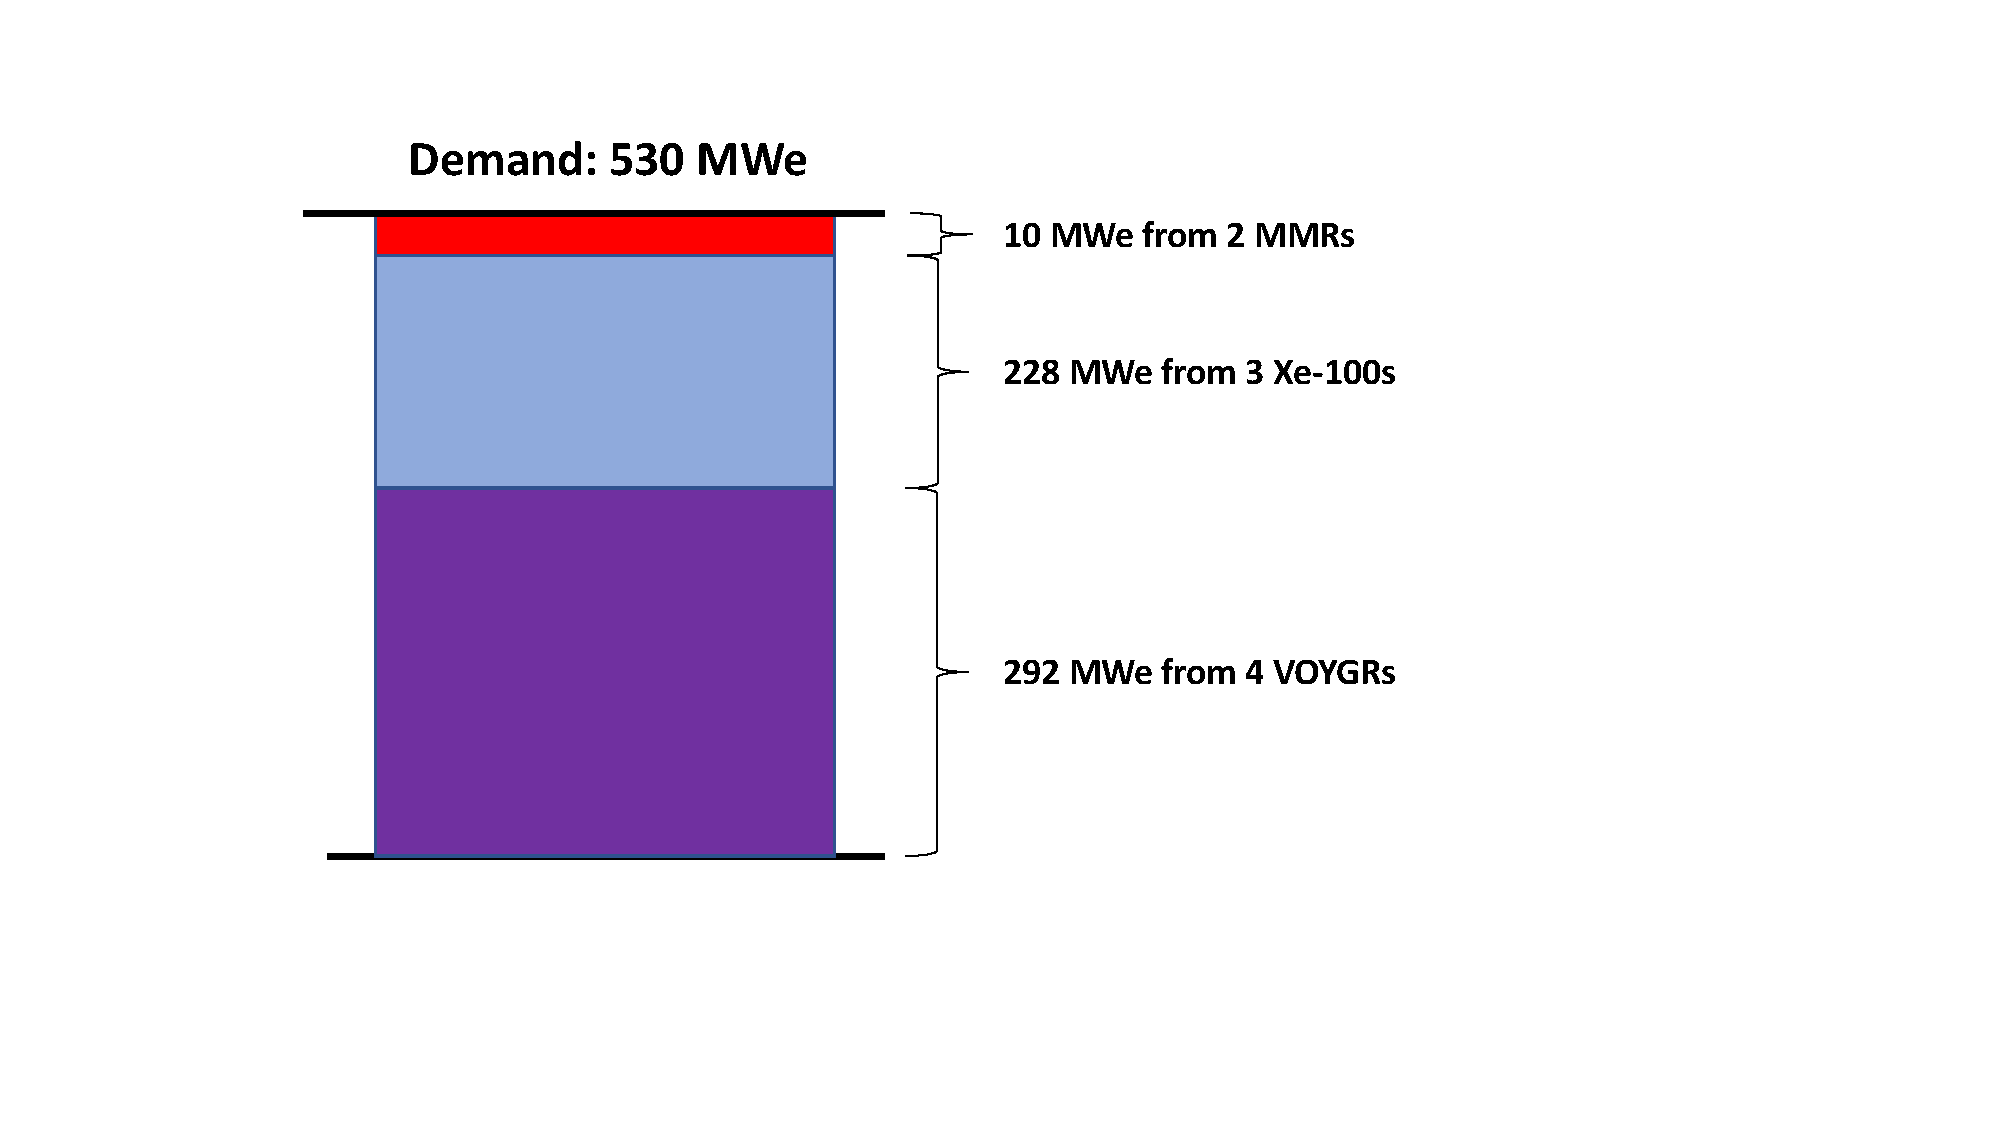
\includegraphics[scale=0.45, trim=50 100 100 0,clip]{VOYGR_build_share.pdf}
    \caption{Demonstration of the adjusted advanced reactor deployment 
    scheme to meet a demand of 530 MWe and a VOYGR build share of 
    50\%.}
    \label{fig:build-share-deploy}
\end{figure}

The \gls{LWR} lifetimes are varied based 
on the percent of the fleet that operate for 60 and 80 years. This 
variable will vary between 0-50\% of the \gls{LWR} fleet operating for 80 
years, while the other \glspl{LWR} operate for 60 years. The 
\glspl{LWR} do not all start operation at the same time, so the 
selection of the \glspl{LWR} that operate for 80 years affects the results, 
even if the number is the same. Therefore, reactors will be selected for 
operation to 80 years in 
descending order of power output, reflecting the greater likelihood of 
larger units receiving a license extension. Previous sensitivity analysis of 
fuel cycle transitions considered the impact of the transition start time 
and the \gls{LWR} lifetimes \cite{chee_sensitivity_2019,feng_sensitivity_2020},
which forms the basis for why these input parameters were selected for this 
work.

Variations of the discharge burnup of each \gls{HALEU}-fueled reactor (the 
Xe-100 and \gls{MMR}) were carried out slightly differently. Variation 
of this parameter is being done because these reactors are aiming to achieve 
burnups that are much higher than what the NRC has approved fuel for 
\hl{Citation?}. Therefore, inclusion of this variable explores the impact 
on resource needs for if these reactors are not able to achieve their 
reported burnups. This analysis is not performed for the VOYGR because this 
design aims to achieve a burnup that the NRC is comfortable with. 

To vary the burnup of the Xe-100, two different systems were enacted. The 
first was to vary the number of passes each pebbles goes through the core
while keeping the length of each pass and the total mass of uranium 
in the core constant. Varying the number of passes between two and six 
results in discharge burnups of 56, 84, 112, 140, and 168 MWd/kgU, 
using Eq. \ref{eq:fuel_mass}. The second system was to vary the length 
of each pass while keeping the number of passes and the total mass of uranium 
constant. The goal of the second system is to cause a small change in the 
discharge burnup to examine how a smaller change in the burnup affects 
the resource needs. This system results in burnups of 151 and 185 MWd/kgU, 
which are about $\pm$10\% of the stated discharge burnup of 168 MWd/kgU. 

To vary the burnup of the \gls{MMR} the cycle time, and thus lifetime, of 
the reactor was varied while the total mass of uranium was held constant. 
Cycle times of 10, 15, and 20 years were considered, resulting in burnup 
values of 41, 62, and 82 MWd/kgU. Additionally, the lifetime was varied to 
result in burnups $\pm$10\% and $\pm$5\% around the stated burnup of 
82 MWd/kg, resulting in burnups of 74, 78, 86, and 90 MWd/kgU. 

The output metrics of 
interest for this analysis include the amount of waste generated that 
must be sent to a repository (\gls{SNF} mass), the mass of enriched uranium, 
the mass of \gls{HALEU},
the amount of \gls{SWU} capacity required to produce all enriched uranium, the 
\gls{SWU} capacity required to produce \gls{HALEU}, and the feed uranium 
required to produce \gls{HALEU}. Each metric will be evaluated based on the 
cumulative sum required, starting at the transition start time. Previous 
sensitivity analysis of fuel cycle transitions considered the waste 
discharged, \gls{SWU} 
capacity required, and natural uranium requirements
\cite{richards_application_2021,feng_sensitivity_2020} 


\section{One-at-a-time}
\subsection{Scenario 7}
This section discusses the results of the \gls{OAT} sensitivity analysis 
as applied to Scenario 7. A subsection of this analysis is presented 
in \hl{Cite ANS Paper}, but the analysis presented here has an expanded scope. 
Additionally, the work presented here uses an updated deployment scheme to 
account for non-consistent replacement of advanced reactors identified in 
\hl{ANS Paper}. The results discuss
the relative change in each metric for each parameter varied. The minimum, 
average, and maximum value for each metric is provided in Table 
\ref{tab:oat_values}.

\begin{table}
    \centering
    \caption{Minimum, average, and maximum value of each metric caused 
    by the variation of each parameter.}
    \label{tab:oat_values}
    \begin{tabular}{llrrr}       
        \hline 
        Parameter &     Metric &      Minimum &      Average &      Maximum \\\hline
        Transition Start &  Fuel Mass & 2.832004e+07 & 3.001442e+07 & 3.085691e+07 \\
                         & HALEU Mass & 2.777396e+07 & 2.931392e+07 & 3.005491e+07 \\ 
                         &  Total SWU & 9.727160e+08 & 1.035603e+09 & 1.067644e+09 \\ 
                         & HALEU SWU & 9.690305e+08 & 1.030876e+09 & 1.062295e+09 \\
                         &        SNF & 2.600173e+07 & 2.743657e+07 & 2.812741e+07 \\  
                         & HALEU Feed & 8.406729e+08 & 8.936249e+08 & 9.204018e+08 \\\hline
        LWR Lifetimes &  Fuel Mass & 2.226230e+07 & 2.574361e+07 & 2.933547e+07 \\
                      & HALEU Mass & 2.186991e+07 & 2.527842e+07 & 2.884623e+07 \\
                      &  Total SWU & 7.779876e+08 & 8.972582e+08 & 1.021053e+09 \\
                      &  HALEU SWU & 7.753394e+08 & 8.941187e+08 & 1.017751e+09 \\
                      &        SNF & 1.955625e+07 & 2.305043e+07 & 2.668538e+07 \\
                      & HALEU Feed & 6.715754e+08 & 7.746336e+08 & 8.819633e+08 \\\hline 
        Xe-100 Build Share &  Fuel Mass & 8.228834e+07 & 1.130189e+08 & 1.471439e+08 \\
                           & HALEU Mass & 2.826681e+06 & 1.077601e+07 & 1.803929e+07 \\
                           &  Total SWU & 1.082813e+09 & 1.089912e+09 & 1.101530e+09 \\
                           &  HALEU SWU & 1.275350e+08 & 3.998760e+08 & 6.501138e+08 \\
                           &        SNF & 7.510853e+07 & 1.032204e+08 & 1.344031e+08 \\
                           & HALEU Feed & 1.081440e+08 & 3.448436e+08 & 5.622094e+08 \\\hline 
        MMR Build Share &  Fuel Mass & 3.701890e+07 & 4.917833e+07 & 6.134049e+07 \\
                        & HALEU Mass & 2.670288e+07 & 3.851759e+07 & 5.039230e+07 \\
                        &  Total SWU & 9.901021e+08 & 1.599871e+09 & 2.211838e+09 \\
                        &  HALEU SWU & 9.204794e+08 & 1.527922e+09 & 2.137948e+09 \\
                        &        SNF & 3.439781e+07 & 4.065525e+07 & 4.688864e+07 \\
                        & HALEU Feed & 7.995188e+08 & 1.309634e+09 & 1.821949e+09 \\\hline 
        VOYGR Build Share &  Fuel Mass & 3.044985e+07 & 6.435525e+07 & 9.510189e+07 \\
                          & HALEU Mass & 1.515573e+07 & 2.233175e+07 & 3.044985e+07 \\
                          &  Total SWU & 1.076518e+09 & 1.082445e+09 & 1.092329e+09 \\
                          &  HALEU SWU & 5.527729e+08 & 7.988284e+08 & 1.079883e+09 \\
                          &        SNF & 2.764653e+07 & 5.870293e+07 & 8.679207e+07 \\
                          & HALEU Feed & 4.774801e+08 & 6.913159e+08 & 9.353306e+08 \\\hline 
        Xe-100 Burnup &  Fuel Mass & 2.760515e+07 & 5.887765e+07 & 1.591116e+08 \\
                      & HALEU Mass & 2.681265e+07 & 5.808515e+07 & 1.583191e+08 \\
                      &  Total SWU & 9.558796e+08 & 2.033879e+09 & 5.489061e+09 \\
                      &  HALEU SWU & 9.505310e+08 & 2.028530e+09 & 5.483713e+09 \\
                      &        SNF & 2.486320e+07 & 5.613569e+07 & 1.563697e+08 \\
                      & HALEU Feed & 8.233245e+08 & 1.759663e+09 & 4.760799e+09 \\\hline 
        MMR Burnup &  Fuel Mass & 3.064950e+07 & 3.123978e+07 & 3.292776e+07 \\
                   & HALEU Mass & 2.985700e+07 & 3.044728e+07 & 3.213526e+07 \\
                   &  Total SWU & 1.058714e+09 & 1.085347e+09 & 1.161506e+09 \\
                   &  HALEU SWU & 1.053366e+09 & 1.079998e+09 & 1.156157e+09 \\
                   &        SNF & 2.790754e+07 & 2.849783e+07 & 3.018581e+07 \\
                   & HALEU Feed & 9.128300e+08 & 9.354133e+08 & 9.999926e+08 \\
        \hline
    \end{tabular}
\end{table}


\subsubsection{Transition start time}
Delays in the transition start time generally decrease all of the output 
metrics, as shown in Figure \ref{fig:ts_scenario7}. This results matches 
expectations, because if the advanced reactors are deployed for less time, 
then they require fewer resources. However, there are some increases in 
the output metrics between individual time steps. For example, a transition 
start time of October 2029 increases the fuel mass and \gls{SNF} mass 
relative to July 2029. This increase is the result of changes in the number 
of each advanced reactor deployed, because of differences in the gap 
between energy produced and energy demand that must initially be filled when 
advanced reactors are deployed. By waiting until October 2029, more VOYGRs 
are deployed than when the transition starts in July 2029. As discussed in 
Chapter \ref{ch:once_through_results}, the VOYGR needs a larger fuel mass, 
and thus discharges more \gls{SNF} than the Xe-100 and \gls{MMR}. Therefore, 
these two metrics increase for this particular transition start time. 

\begin{figure}
    \centering
    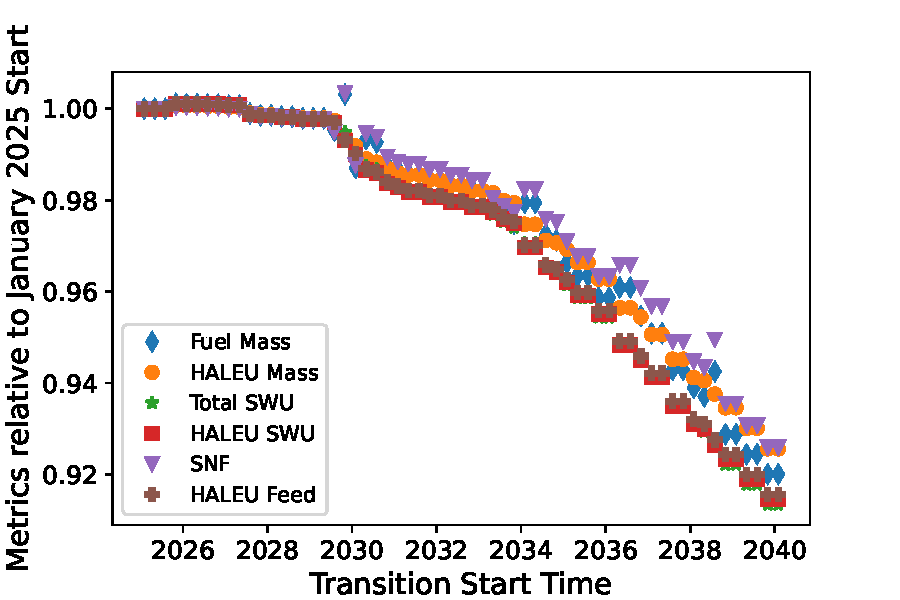
\includegraphics[scale=0.8]{ts.pdf}
    \caption{Change in each metric as a function of transition start 
    time, relative to a transition start in January 2025.}
    \label{fig:ts_scenario7}
\end{figure}

The \gls{HALEU} mass required for these transitions varied between 27.8-30.9
MTU. 

One of the disadvantages in delaying the transition start time is the 
increasing gap between energy supplied and energy demand as the transition 
start time is delayed. All of these scenarios have a constant demand 
of 87.20 GWe-yr beginning in 2025. By delaying the transition start time 
to after September 2025 (the observed initial deployment time of advanced 
reactors in Section \ref{sec:nogrowth_reactors}) there is some gap between 
the energy supplied and the energy demand. The largest gap observed is 36.7
GWe-yr, when reactors are deployed starting in January 2040. This difference 
between energy supplied and energy demand is a disadvantage of delaying 
the start time to reduce material requirements. 

\subsubsection{LWR lifetimes}
The next metric varied is the percent of the \glspl{LWR} that operate for 
80 years, reflecting a license extension. As the percent of the \gls{LWR} 
fleet operating for 80 years increases all of the metrics decrease, as 
Figure \ref{fig:lwr_scenario7} shows. All of the metrics decrease by a similar 
magnitude, with some variation because of changes in the number of each advanced 
reactor deployed, as previously discussed. The \gls{SNF} mass decreases more 
than the other metrics across this parameter space, ranging between 
19.5-26.7 MTU.

\begin{figure}
    \centering
    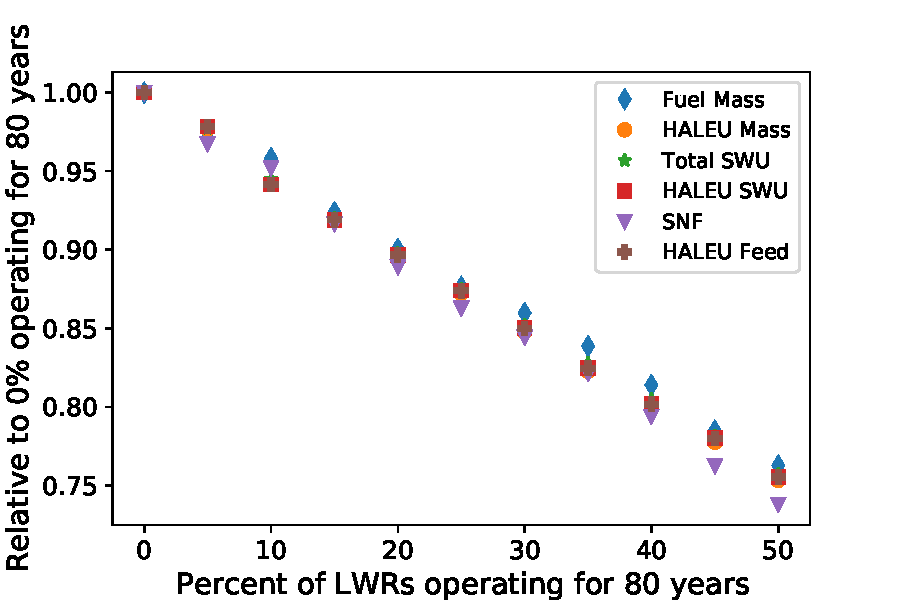
\includegraphics[scale=0.8]{lwr.pdf}
    \caption{Change in each metric as a function of percent of LWR fleet  
    operating for 80 years, relative to 0\%.}
    \label{fig:lwr_scenario7}
\end{figure}

Across this parameter space, the metrics decrease by a greater fraction than 
when varying the transition start time. The increased impact on the metrics 
is partly because the \glspl{LWR} that don't operate for 80 years all operate for 
60 years when varying this parameter, but not all of the \glspl{LWR} operate for 
60 years in the initial transition analysis or when varying the transition
start time. This modeling difference, made to simplify defining the advanced 
reactor deployment schedule, does not have a large impact on the results as 
evidenced by the maximum \gls{HALEU} mass when varying the \gls{LWR} lifetimes 
being only 4.9\% lower than the maximum \gls{HALEU} mass when varying the 
transition start time. This minimal impact from the modeling difference is 
because most of the \glspl{LWR} operate for 60 years when varying the transition start 
time. Therefore, we can attribute most of the change in the metrics to the 
change in the \gls{LWR} lifetimes. In addition to causing greater change in 
the metrics, the energy demand is always met when varying the \gls{LWR} lifetimes,
which suggests that extending the lifetimes of the \glspl{LWR} is a better 
parameter to vary if one wishes to decrease material requirements of this 
transition. 

\subsubsection{Xe-100 build share}
As the Xe-100 build share increases, the \gls{HALEU}-related metrics 
increase while the total \gls{SNF} and total fuel mass decrease and the 
total \gls{SWU} capacity stays relatively constant (Figure \ref{fig:xe100_scenario7}).
As Figure \ref{fig:xe100_s7_combined_reactors} shows, as the Xe-100 build share 
increases, the number of \glspl{MMR} is relatively constant and the number of 
VOYGRs decreases. These results show that as the Xe-100 build share increases, they 
are primarily replacing power that is supplied by the VOYGRs, instead of a portion 
of each of the other advanced reactors. This replacement of VOYGRs is because 
of the deployment scheme of this work, as the VOYGR has the largest power output 
between the VOYGR and \gls{MMR}. Therefore, the VOYGR is primarily deployed when 
the Xe-100 build share is 0\%. 

\begin{figure}
    \centering
    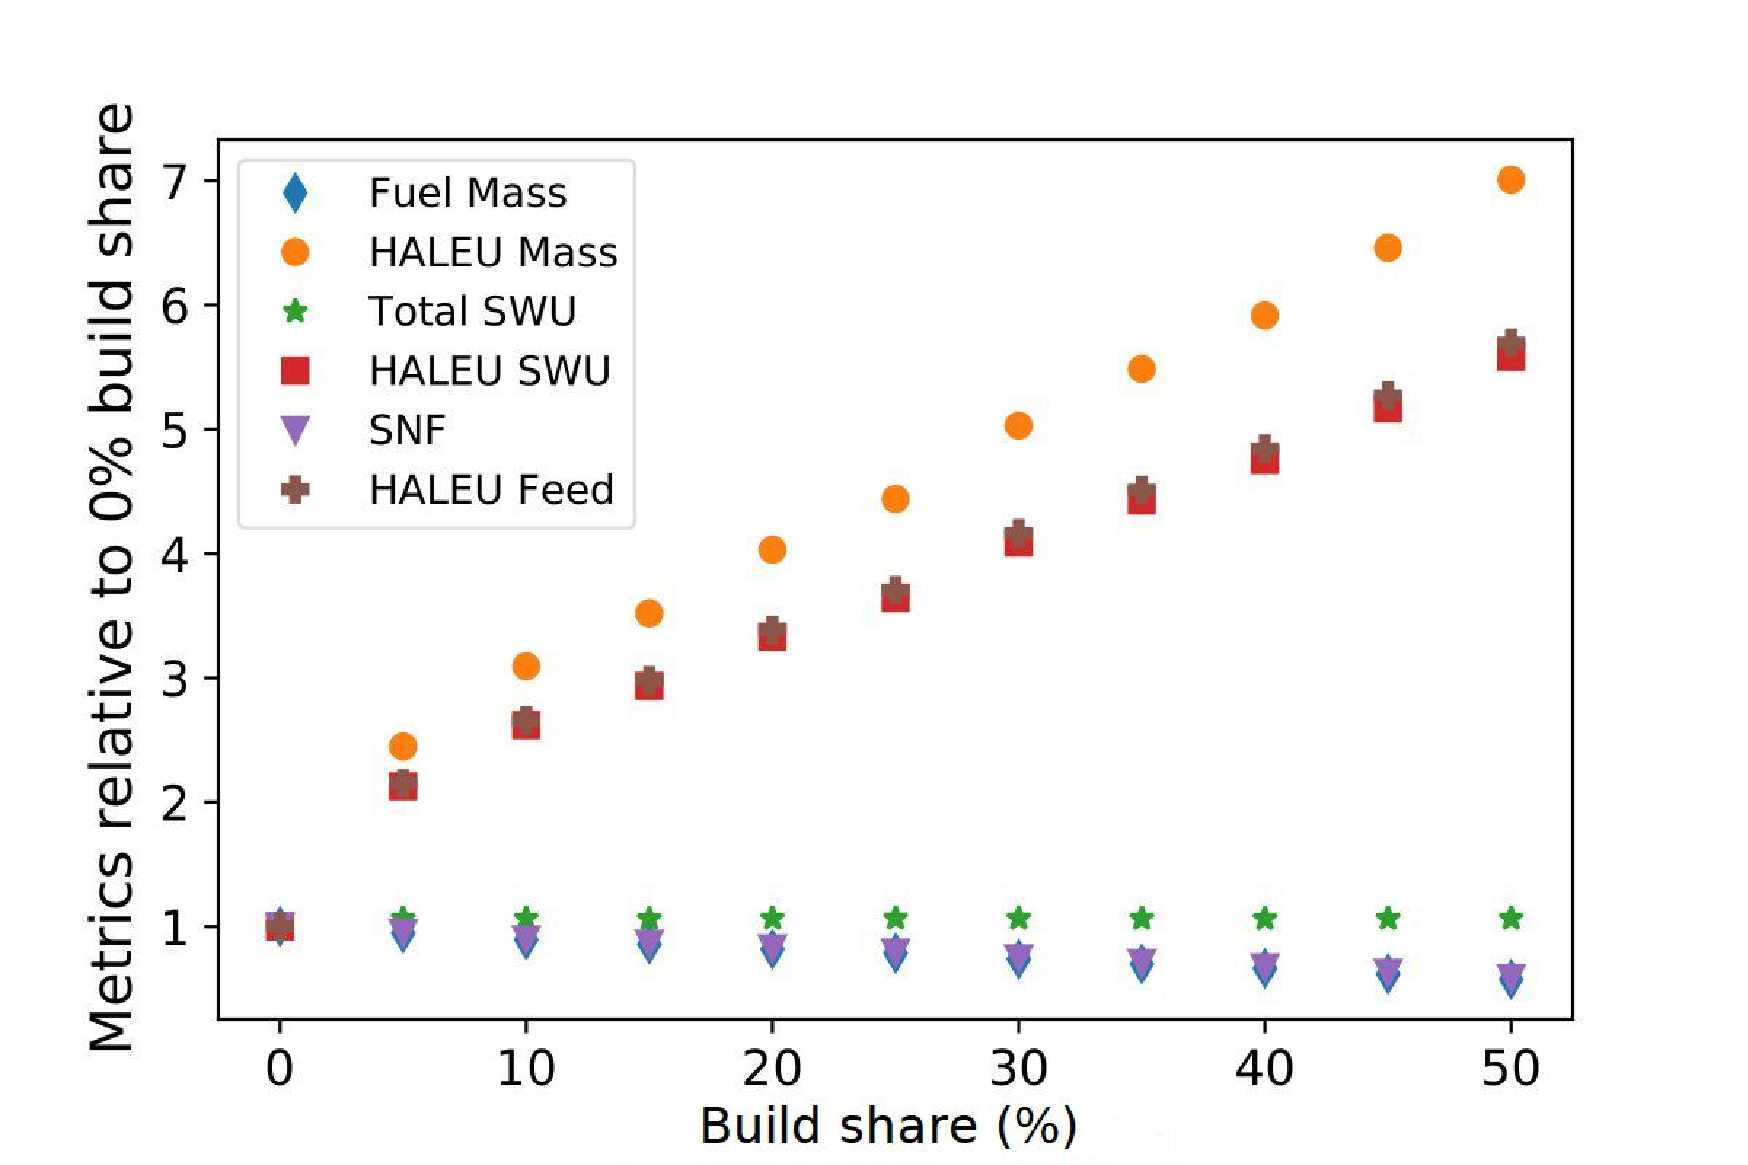
\includegraphics[scale=0.8]{xe100.pdf}
    \caption{Change in each metric as a function of Xe-100 build share, 
    relative to a build share of 0\%.}
    \label{fig:xe100_scenario7}
\end{figure}

\begin{figure}
    \centering
    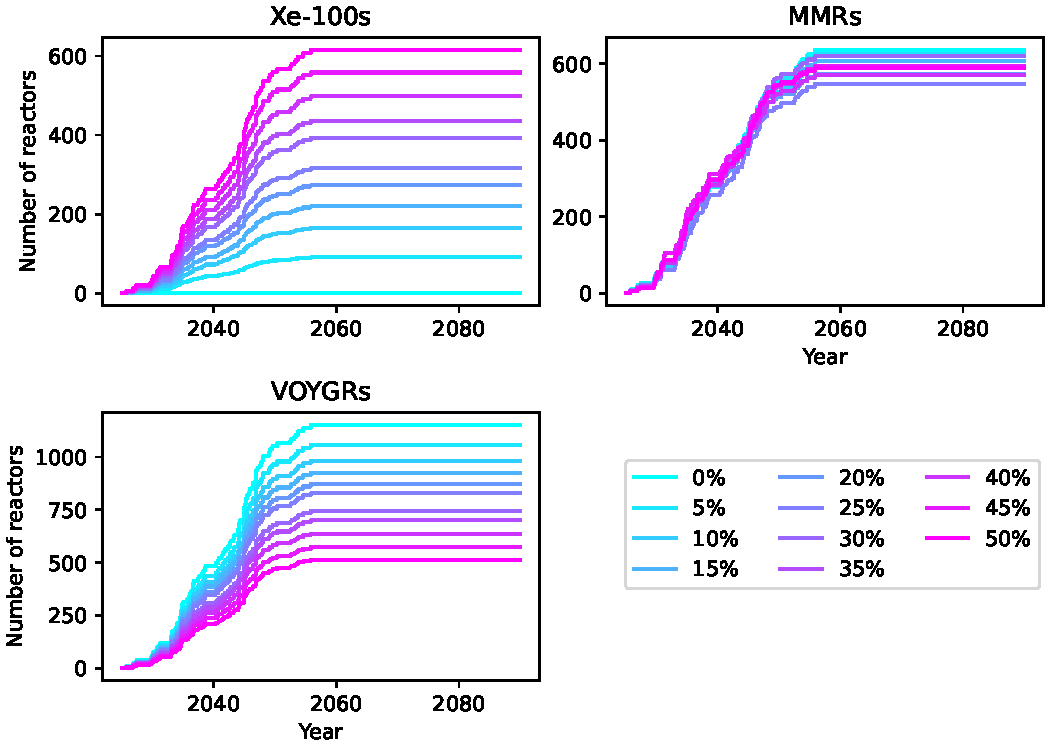
\includegraphics[scale=0.7]{xe100_combined_reactors.pdf}
    \caption{Number of Xe-100s (top left), MMRs (top right), and VOYGRs
    (bottom left) as a function of Xe-100 build share.}
    \label{fig:xe100_s7_combined_reactors}
\end{figure}

The \gls{HALEU}-related metrics increase with Xe-100 build share because more the 
power comes from advanced reactors requiring \gls{HALEU}. The total fuel mass and 
\gls{SNF} mass decrease because the Xe-100s are primarily replacing VOYGRs, and the 
Xe-100 requires less fuel per unit time and energy than the VOYGR, as discussed 
in Chapter \ref{ch:once_through_results}. The total \gls{SWU} capacity required 
is relatively constant, decreasing between 0.3-1.7\% compared to the \gls{SWU} capacity 
required for a 0\% Xe-100 build share. This stagnant behavior of the total 
\gls{SWU} capacity is consistent with the similar \gls{SWU} capacity required 
by Scenarios 3-7 in Section \ref{sec:nogrowth_swu}, when either the Xe-100 or 
VOYGR are primarily deployed. These results highlight the trade-off between the
\gls{HALEU}-related metrics and the total fuel mass and \gls{SNF} mass in deploying 
the Xe-100 versus the VOYGR. Both reactors require similar \gls{SWU} capacities, 
but because of the different product assays required the cascade configuration 
will vary. 

The \gls{HALEU}-related metrics increase to up to 538.2\% of the mass required 
for a 0\% Xe-100 build share. The total fuel mass and \gls{SNF} mass decrease 
to up to 44.11\% of the mass required for 1 0\% Xe-100 build share. 


\subsubsection{MMR build share}
As the \gls{MMR} build share increases all of the metrics increase, as shown 
in Figure \ref{fig:mmr_scenario7}. As Figure \ref{fig:mmr_reactors_s7} shows, 
as the \gls{MMR} build share increases, the number of Xe-100s decreases, the 
number of \glspl{MMR} increases, and the number of VOYGRs is relatively constant. 
Therefore, variation in the \gls{MMR} build share highlights the results of 
deploying \glspl{MMR} over the Xe-100. 

\begin{figure}
    \centering
    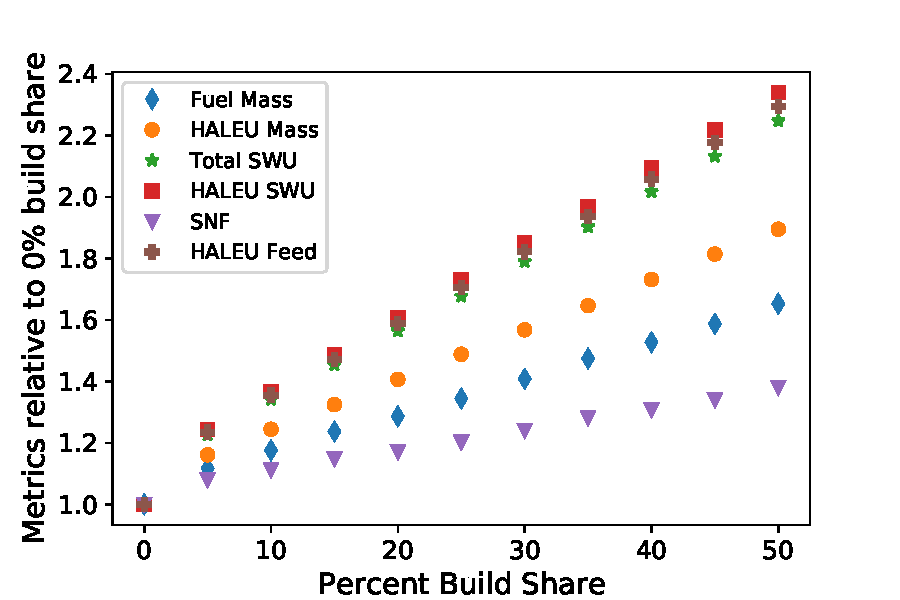
\includegraphics[scale=0.8]{mmr.pdf}
    \caption{Change in each metric as a function of MMR build share, 
    relative to a build share of 0\%.}
    \label{fig:mmr_scenario7}
\end{figure}


\begin{figure}
    \centering
    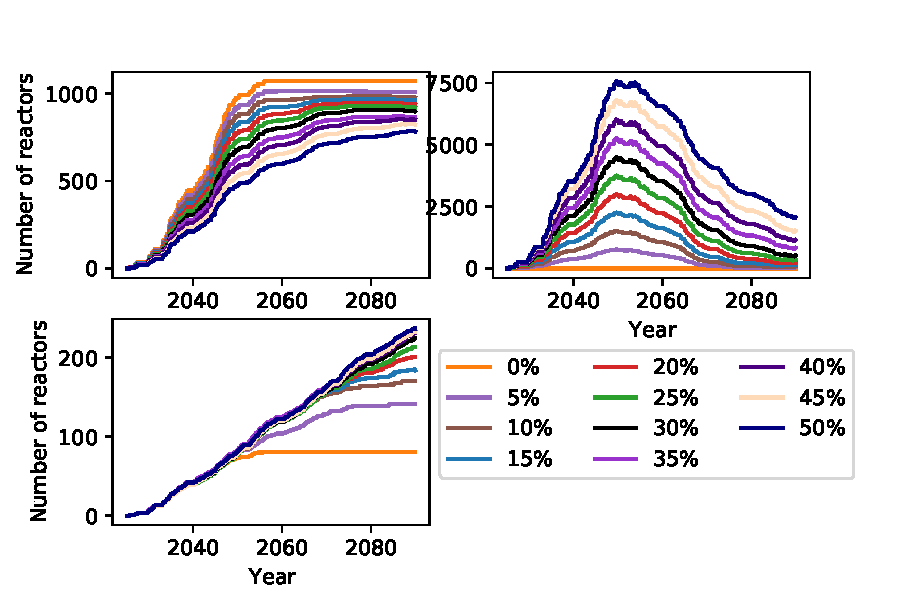
\includegraphics[scale=0.7]{mmr_combined_reactors.pdf}
    \caption{Number of Xe-100s (top left), MMRs (top right), and 
    VOYGRs (bottom left) deployed as a function of time and 
    MMR build share.}
    \label{fig:mmr_reactors_s7}
\end{figure}

All of the metrics increase because the \gls{MMR} requires more fuel and 
a higher product assay than the Xe-100. 
The total \gls{SWU}, \gls{SWU} to produce \gls{HALEU}, and feed to 
produce \gls{HALEU} experience the greatest relative increase as the 
\gls{MMR} build share increases. These metrics all increase the most 
because the increase in the product assay is compounded with the increase 
in the product mass when calculating these three metrics. 


\subsubsection{VOYGR build share}
When varying VOYGR build share, the impact on the metrics was 
opposite that of when varying the Xe-100 build share (Figure 
\ref{fig:voygr_scenario7}). The total fuel mass and \gls{SNF} mass 
increase, the \gls{HALEU}-related metrics decrease, and the total 
\gls{SWU} capacity remains relatively constant. This reversal 
of trends occurs because there is a replacement of Xe-100s with VOYGRs
with increasing build share, 
the opposite of what happens with an increasing Xe-100 build share. 

\begin{figure}
    \centering
    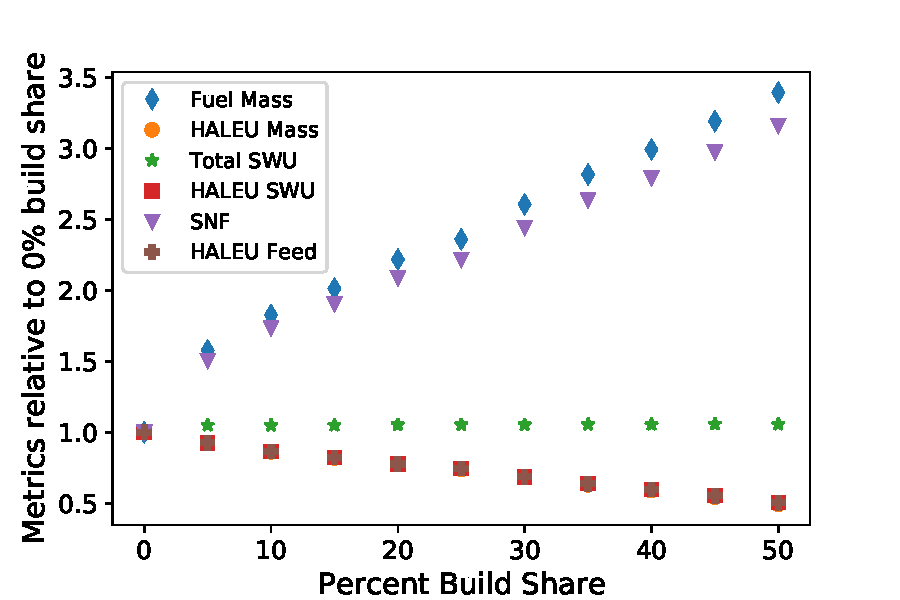
\includegraphics[scale=0.8]{voygr.pdf}
    \caption{Change in each metric as a function of VOYGR build share, 
    relative to a build share of 0\%.}
    \label{fig:voygr_scenario7}
\end{figure}

The total \gls{SWU} capacity required varies between 99.6\%-101.2\% of the 
\gls{SWU} capacity needed for a 0\% VOYGR build share, a range of 1.077$\times 10^9$
- 1.092$\times 10^9$ kg-SWU. The total fuel mass and \gls{SNF} mass increase 
up to 313.9\% of the mass required for a 0\% VOYGR build share, and the 
\gls{HALEU}-related metrics decrease to 49.77\% of the mass required 
for a 0\% VOYGR build share. While the trends from varying the VOYGR build share 
mirrors the trends from varying the Xe-100 build share, the magnitude of the 
changes are not the same. This magnitude difference is because the variations 
in these parameters does covers adjacent but not overlapping design spaces. 

\subsubsection{Xe-100 burnup}
When varying the burnup of fuel discharged from Xe-100s, the metrics decrease 
as the burnup increases (Figure \ref{fig:xe100_bu_s7}). This decrease in material requirements because as 
the burnup is increased the fuel is going through the core more times or the 
length of each pass is longer. Therefore, the Xe-100s in the simulation are receiving 
less fuel at each refueling or receiving fuel less often as the burnup increases. 
Varying the burnup of the Xe-100 has a large impact on the metrics, up to fives times 
the material requirements compared with a burnup of 168 MWd/kgU, because most of 
the energy produced in these scenarios comes from Xe-100s and many more Xe-100s are 
deployed than \glspl{MMR} or VOYGRs. Therefore, changes to the Xe-100 refueling is 
magnified because of the greater number of the reactor deployed. 

\begin{figure}
    \centering
    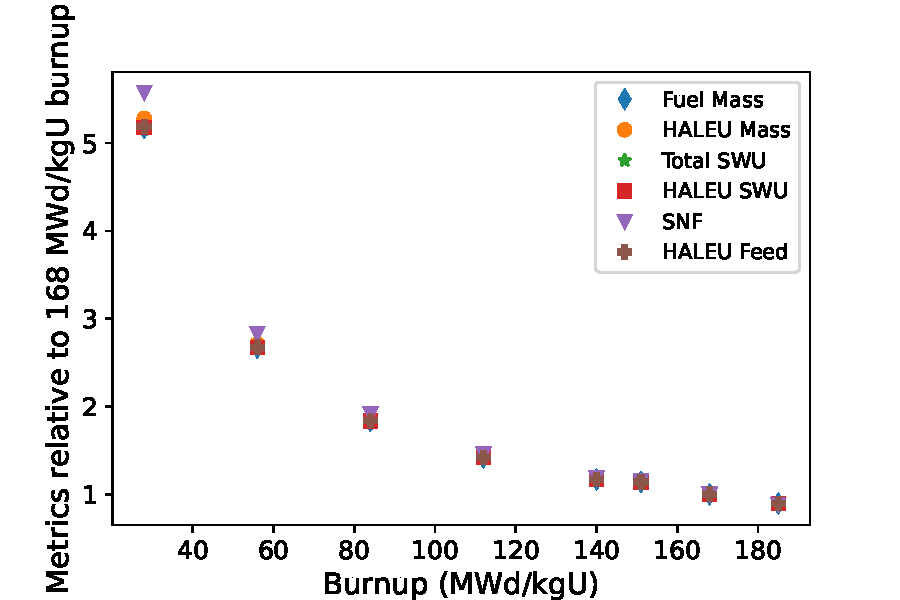
\includegraphics[scale=0.8]{xe100_bu.pdf}
    \caption{Change in metrics from varying the burnup of fuel 
    discharged from Xe-100, relative to a burnup of 168 MWd/kgU.}
    \label{fig:xe100_bu_s7}
\end{figure}

\subsubsection{MMR burnup}
When the \gls{MMR} discharge burnup is varied the metrics all decrease, similar 
to what was observed by varying the Xe-100 discharge burnup. One difference in 
the trends observed between varying these two parameters is the magnitude of 
the relative changes. Varying the \gls{MMR} burnup has a smaller relative effect 
on the metrics than varying the Xe-100 burnup because there are fewer \glspl{MMR} 
deployed in the transition. Therefore the impact on the cumulative metrics 
(what is reported here) is smaller. Another difference is that the total 
\gls{SWU}, \gls{HALEU} \gls{SWU}, and \gls{HALEU} feed increase the most 
when the \gls{MMR} burnup is low, compared with the \gls{SNF} having the 
greatest relative increase with the Xe-100 burnup is low. 

\begin{figure}
    \centering
    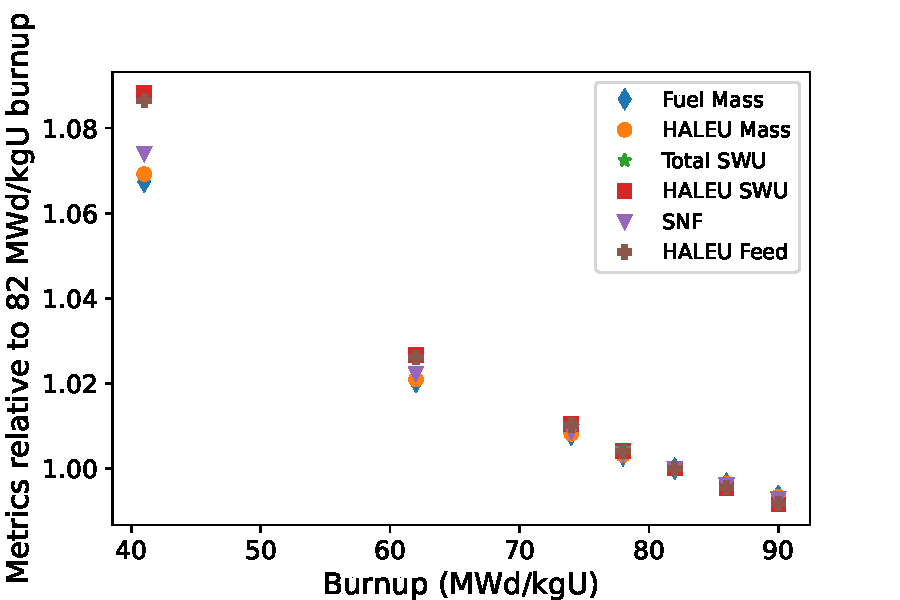
\includegraphics[scale=0.8]{mmr_bu.pdf}
    \caption{Change in metrics from varying the burnup of fuel 
    discharged from the MMR, relative to a burnup of 82 MWd/kgU.}
    \label{fig:mmr_bu_s7}
\end{figure}

\subsubsection{Burnup variations with a common build share}
To better investigate the effect of varying the discharge burnup of the Xe-100 
and \gls{MMR} without the influence of the deployment scheme preferentially
deploying Xe-100s, we repeated each set of analysis using a constant 20\% 
build share for the Xe-100 and \gls{MMR}. Using a constant build share for 
both reactors means that they each will supply the same fraction of the energy demand.
However, because of the different power output for each reactor a constant build 
share does not mean that the same number of each reactor is built. 

\subsection{Scenario 14}

\section{Synergistic}
The synergistic analysis in this work varied two parameters at a time to 
investigate some of the combined effects of the input parameters. Synergistic 
sensitivity analysis helps to identify if the combined effect of two parameters 
has a greater impact on the metrics that when varying a single parameter. 

\subsection{Scenario 7}
We ran synergistic 
analysis on all combinations of two input parameters studied in the \gls{OAT} 
analysis, except combinations of two specified build shares. The
results presented here are only a small subsection of the analysis performed, 
with the remaining results in Appendix \ref{app:s7_synergistic}.

\subsubsection{LWR lifetime and VOYGR build share}
When the percent of \glspl{LWR} operating for 80 years and the VOYGR build share 
were varied, the results are consistent with the results from varying 
each of the parameters by themselves. The effect on the \gls{HALEU} mass 
(Figure \ref{fig:lwr_voygr_share_enr_u})

\begin{figure}[ht]
    \centering
    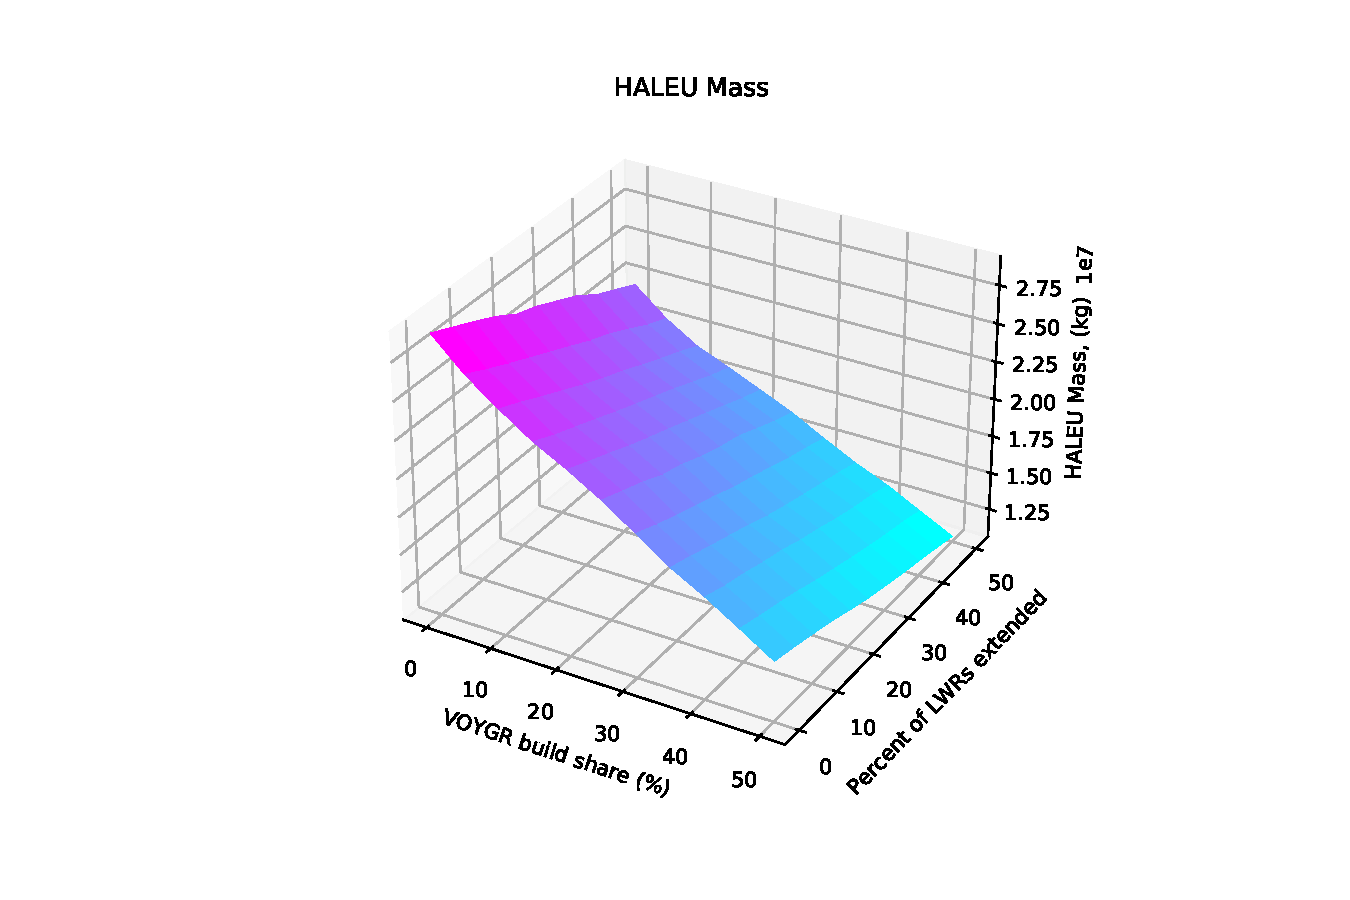
\includegraphics[width=\textwidth, trim=120 0 120 0, clip]{lwr_voygr_share_haleu.pdf}
    \caption{Effect on HALEU mass.}
    \label{fig:lwr_voygr_share_haleu}
\end{figure}

\subsubsection{Xe-100 build share and Xe-100 burnup}

\subsubsection{Xe-100 build share and MMR burnup}

\subsubsection{Transition start and Xe-100 build share}

\subsubsection{Transition start and MMR build share}

\subsection{Scenario 14}

\section{Global}
\subsection{Scenario 7}

\subsection{Scenario 14}


